%
\begin{figure}
\begin{center}
\usetikzlibrary{automata, positioning}
    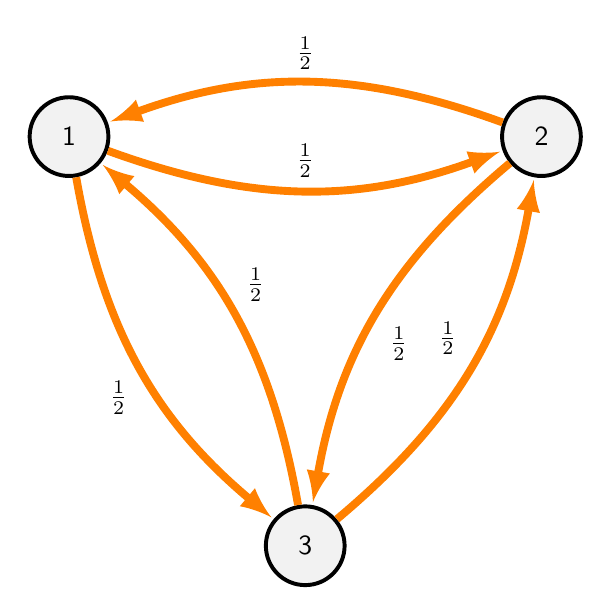
\begin{tikzpicture}[font=\sffamily]
        % Setup the style for the states
        \tikzset{node style/.style={state, 
                                    minimum width=1cm,
                                    line width=0.5mm,
                                    fill=gray!10!white}}

        % Draw the states
        \node[node style] at (0, 0)     (1)     {1};
        \node[node style] at (6, 0)     (2)     {2};
        \node[node style] at (3, -5.196) (3) 	{3};

        % Connect the states with arrows
        \draw[every loop,
              auto=right,
              line width=1mm,
              >=latex,
              draw=orange,
              fill=orange]
            (1)     edge[bend right=20]            node {$\frac{1}{2}$} (3)
            (1)     edge[bend right=20, auto=left] node {$\frac{1}{2}$} (2)
            (2)     edge[bend right=20]            node {$\frac{1}{2}$} (1)
            (2)     edge[bend right=20, auto=left] node {$\frac{1}{2}$} (3)
            (3) edge[bend right=20]            node {$\frac{1}{2}$} (1)
            (3) edge[bend right=20, auto=left] node {$\frac{1}{2}$} (2);
    \end{tikzpicture}  
    \caption{State transition diagram}
\end{center}
    \end{figure}    
    \begin{enumerate}
    \item{ The period of state 1 i.e, $d(1)$ is given as:
    \begin{align}
    d(1)=GCD\{n : P_{11}^n > 0\} \label{eq:solutions/2018/june/105/eq1a}
    \end{align}
     For $n=1$,
    \begin{align}
    \vec{P}=\myvec{0&\frac{1}{2}&\frac{1}{2}\\\frac{1}{2}&0&\frac{1}{2}\\\frac{1}{2}&\frac{1}{2}&0}\\
    \end{align}
    For $n=2$,
    \begin{align}
    \vec{P}^2=\myvec{\frac{1}{2}&\frac{1}{4}&\frac{1}{4}\\\frac{1}{4}&\frac{1}{2}&\frac{1}{4}\\\frac{1}{4}&\frac{1}{4}&\frac{1}{2}}\\
    \end{align}
    For $n=3$,
    \begin{align}
    \vec{P}^3=\myvec{\frac{1}{4}&\frac{3}{8}&\frac{3}{8}\\\frac{3}{8}&\frac{1}{4}&\frac{3}{8}\\\frac{3}{8}&\frac{3}{8}&\frac{1}{4}}\\
    \end{align}
        For $n=4$,
    \begin{align}
    \vec{P}^4=\myvec{\frac{3}{8}&\frac{5}{16}&\frac{5}{16}\\\frac{5}{16}&\frac{3}{8}&\frac{5}{16}\\\frac{5}{16}&\frac{5}{16}&\frac{3}{8}}
    \end{align}
Thus $P_{11}^n$ follows the sequence, that is defined as:
\begin{align}
    P_{11}^n= 
\begin{cases}
	0,& \text{if } n=1\\
    \frac{1}{2},& \text{if } n=2\\
    \frac{1}{2}(P_{11}^{n-1}+P_{11}^{n-2}),& \text{if } n >2
\end{cases}
\end{align}
    Since, for $n>1$, $P_{11}^n>0$
    \begin{align}
    d(1)=GCD\{2,3,4,5\cdots\}\\
    \therefore d(1)=1 \label{eq:solutions/2018/june/105/eq1}
    \end{align}
    Thus statement a is correct}\\
    \item{As calucalted above in \ref{eq:solutions/2018/june/105/eq1}, $d(1)=1$\\
    Thus statement b is incorrect.}\\
    \item{For stationary distribution,
    \begin{align}
    &\sum_{i=1}^{i=n} \pi_i = 1 \\
    &\implies\myvec{1&1&1}\myvec{\pi_1\\\pi_2\\\pi_3}=1\label{eq:solutions/2018/june/105/eq2}
    \end{align}
    Also for a stationary distribution,
    \begin{align}
    &\pi \vec{P} = \pi \\
    &(\pi \vec{P})^T = \pi^T \\
    &\vec{P}^T\pi^T=\pi^T\\
    &\implies (\vec{P}^T-\vec{I})\pi^T=0\\
    &\myvec{-1&\frac{1}{2}&\frac{1}{2}\\\frac{1}{2}&-1&\frac{1}{2}\\\frac{1}{2}&\frac{1}{2}&-1}\myvec{\pi_1\\\pi_2\\\pi_3}=\myvec{\pi_1\\\pi_2\\\pi_3} \label{eq:solutions/2018/june/105/eq3}  
\end{align}
    The given equation \ref{eq:solutions/2018/june/105/eq2}, \ref{eq:solutions/2018/june/105/eq3} can be written as:\\
    \begin{align}
    \myvec{-1&\frac{1}{2}&\frac{1}{2}\\\frac{1}{2}&-1&\frac{1}{2}\\\frac{1}{2}&\frac{1}{2}&-1\\1&1&1}\myvec{\pi_1\\\pi_2\\\pi_3}=\myvec{0\\0\\0\\1}
    \end{align}
    We need to solve the augmented matrix to row reduced echelon form to get the solution,    
    \begin{align}
    \myvec{-1&\frac{1}{2}&\frac{1}{2}&\vrule&0\\\frac{1}{2}&-1&\frac{1}{2}&\vrule&0\\\frac{1}{2}&\frac{1}{2}&-1&\vrule&0\\1&1&1&\vrule&1}\xleftrightarrow{R_4=R_4+R_1}\\\myvec{-1&\frac{1}{2}&\frac{1}{2}&\vrule&0\\\frac{1}{2}&-1&\frac{1}{2}&\vrule&0\\\frac{1}{2}&\frac{1}{2}&-1&\vrule&0\\0&\frac{3}{2}&\frac{3}{2}&\vrule&1}\xleftrightarrow{R_1=-R_1}\\\myvec{1&-\frac{1}{2}&-\frac{1}{2}&\vrule&0\\\frac{1}{2}&-1&\frac{1}{2}&\vrule&0\\\frac{1}{2}&\frac{1}{2}&-1&\vrule&0\\0&\frac{3}{2}&\frac{3}{2}&\vrule&1}\xleftrightarrow{R_2=R_2-\frac{R_1}{2}, R_3=R_3-\frac{R_1}{2}}\\\myvec{1&-\frac{1}{2}&-\frac{1}{2}&\vrule&0\\0&-\frac{3}{4}&\frac{3}{4}&\vrule&0\\0&\frac{3}{4}&-\frac{3}{4}&\vrule&0\\0&\frac{3}{2}&\frac{3}{2}&\vrule&1}\xleftrightarrow{R_3=R_3+R_2, R_4=R_4+2R_2}\\\myvec{1&-\frac{1}{2}&-\frac{1}{2}&\vrule&0\\0&-\frac{3}{4}&\frac{3}{4}&\vrule&0\\0&0&0&\vrule&0\\0&0&3&\vrule&1}\xleftrightarrow{R_2=-\frac{4}{3}R_2}\\\myvec{1&-\frac{1}{2}&-\frac{1}{2}&\vrule&0\\0&1&-1&\vrule&0\\0&0&0&\vrule&0\\0&0&3&\vrule&1}\xleftrightarrow{R_1=R_1+\frac{1}{2}R_2}\\\myvec{1&0&-1&\vrule&0\\0&1&-1&\vrule&0\\0&0&0&\vrule&0\\0&0&3&\vrule&1}\xleftrightarrow{R_3 \leftrightarrow R_4}\\\myvec{1&0&-1&\vrule&0\\0&1&-1&\vrule&0\\0&0&3&\vrule&1\\0&0&0&\vrule&0}\xleftrightarrow{R_3=\frac{R_3}{3}}\\\myvec{1&0&-1&\vrule&0\\0&1&-1&\vrule&0\\0&0&1&\vrule&\frac{1}{3}\\0&0&0&\vrule&0}\xleftrightarrow{R_1=R_1+R_3, R_2=R_2+R_3}\\\myvec{1&0&0&\vrule&\frac{1}{3}\\0&1&0&\vrule&\frac{1}{3}\\0&0&1&\vrule&\frac{1}{3}\\0&0&0&\vrule&0}
    \end{align}
    Hence,
    \begin{align}
    \pi_1=\pi_2=\pi_3=\frac{1}{3} \label{eq:solutions/2018/june/105/eq10}
    \end{align}
    Thus statement c is incorrect
    }\\
    \item{As, calculated in \ref{eq:solutions/2018/june/105/eq10}, $\pi_1=\frac{1}{3}$\\
    Thus statement d is correct}
    \end{enumerate}
Hence, statements a and d are correct.
